\documentclass{article}
\usepackage{graphicx}
\usepackage{titlesec}
\usepackage{hyperref}
\usepackage{enumitem}
\usepackage{lmodern}
\usepackage{amsmath}
\usepackage{fancyhdr}
\usepackage{textcomp}
\usepackage{lmodern}% http://ctan.org/pkg/lm
\usepackage[table,x11names,svgnames]{xcolor}
\usepackage{soul}
\usepackage{parskip}
\usepackage{multirow}
\usepackage{array}
\usepackage{chngcntr}
\usepackage{afterpage}
\usepackage{tabularx}
\usepackage{float}
\usepackage{placeins}
\usepackage{tablefootnote}
\usepackage{microtype}
\usepackage{textcomp}
\usepackage{titlesec}
\usepackage{enumitem}
\usepackage{listings}
\usepackage{subcaption}
\usepackage{verbatim}
\usepackage[htt]{hyphenat}
\usepackage[letterpaper, portrait, margin=1.5in]{geometry}
\counterwithin{table}{section}
\counterwithin{figure}{section}

% Directives
\setlength\extrarowheight{5pt}

\setcounter{secnumdepth}{4}
\titleformat{\paragraph}
{\normalfont\normalsize\bfseries}{\theparagraph}{1em}{}

\begin{document}

\hrulefill \par
{\Large \textbf{Plant leaf classification}\par}
{\Large Project Milestone\par}
\hrulefill \par
\begin{align*}
\mathrm{Albert\ Liu}
  &&\href{mailto:albertpl@stanford.edu}{albertpl@stanford.edu}\\
\mathrm{Yangming\ Huang}
  &&\href{mailto:yangming@stanford.edu@standford.edu}{yangming@stanford.edu}\\
\end{align*}

\section{ Introduction } 
We have considered the following approaches after literature study.
\begin{enumerate}
  \item Local descriptors + Bag of Features (BoF)\\
   Due to the simplicity and performance, this well established approach was taken at first. Interest points are detected from the raw images and then local invariant feature descriptors are collected, which are clustered to form the visual vocabulary/codebook. Afterwards, each raw image can be represented with histograms of visual words, i.e. term vectors. 
 \item Global shape feature descriptors\\
   Instead of describing the patches of image, the image, as a whole, can be represented with a global description. In the context of plant classification, the shape is considered the most distinct characteristics \cite{Itheri}, among other types of descriptions, i.e., color and texture.
\end{enumerate}
In both cases, the new image representations can be used to train classifiers of our choices.


\section{Data set}
We found these datasets.
\begin{enumerate}
  \item UCI leaf dataset \cite{UCIDataSet}: 40 species with 5 to 16 samples per specie
  \item Kaggle leaf dataset\cite{Pedro13}: 99 species with 16 samples per specie
  \item Swedish leaf dataset \cite{SwedishLeafDataset}: 15 species with 952 samples (roughly 60 samples per specie)
  \item Flavia leaf dataset \cite{FlaviaDataset}: 33 species with roughly 60 samples per specie
  \item Pl@ntNet \cite{PlanetNet}: the most challenging dataset as images are collected through crowd sourced application. 71 species with 5436 images.

\end{enumerate}

\section{Status}
We have prototyped a BoF system, based on OpenCV package, and test with the Swedish dataset \cite{SwedishLeafDataset}. Here is the illustration of the system \ref{fig:bofsystemdesign}.
\begin{figure} 
  \centering
  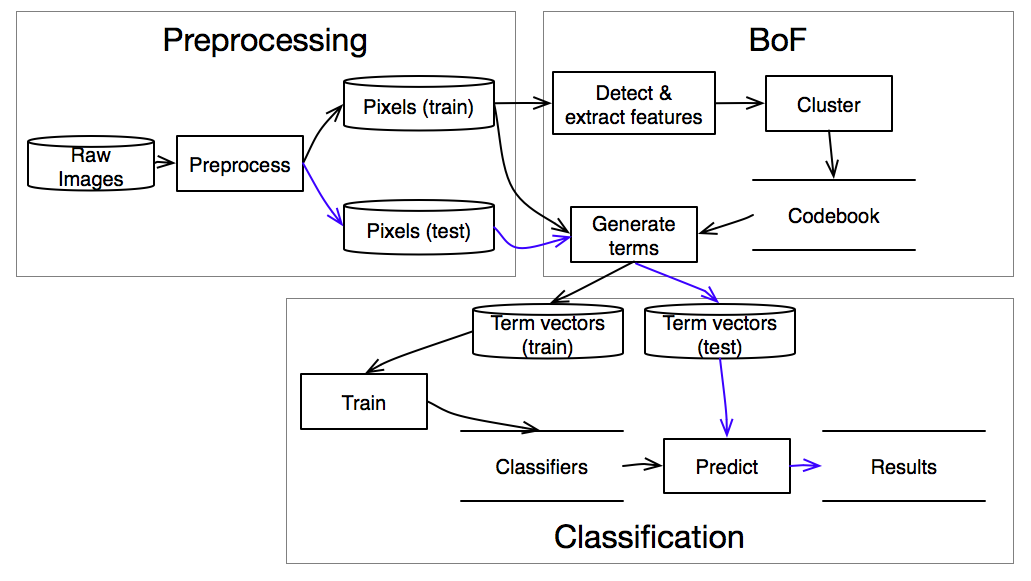
\includegraphics[width=\textwidth]{flowchart}
  \caption{ System Design for BoF }
  \label{fig:bofsystemdesign}
\end{figure}
During preprocessing, raw images are converted to gray-scaled images and resized to reduce computation complexity. We extract SIFT descriptors from the pixels after detecting the key points. Limiting the width of image to 128 pixels, we have roughly 200 SIFT descriptors per image. Then all the descriptors are clustered to build visual words via K-Means. Due to computation complexity, we pick randomly 100 training images to build the visual vocabulary for the initial run.  Here are the preliminary results \ref{table:prelimaryresult}
\begin{table}
  \caption {preliminary test accuracy of BoF approach on Swedish dataset}
  \centering
  \begin{tabular} { c c c c}
    \hline\hline
    Vocabulary size & Softmax &  Linear SVM  & RBF SVM \\
    \hline
    100  &  0.86 & 0.86 & 0.87\\
    1000 &  0.93 & 0.93 & 0.93 \\
    2500 &  0.93 & 0.94 & 0.94 \\
    \hline
  \end{tabular}
  \label{table:prelimaryresult}
\end{table}


We look at the results and notice
\begin{enumerate}
  \item Since there are large features relative to training set, we are not surprised that SVM with linear kernel and Softmax perform well. 
  \item The test accuracy is improved with larger vocabulary size. This makes sense since the more granularity the local descriptors are, the better they could represent the discriminative characteristics.
\end{enumerate}

\section{TODO}
\begin{enumerate}
  \item We will work on the global descriptor approach and then compare the pro and con between these two approaches.
  \item Swedish data set is high quality dataset with large samples per species and we will test our BoF system with more challenging data set. We expect worse test results and this will give us motivation to enhance our system.
  \item We reduce the total number of local descriptors for build the vocabulary by limiting the samples. We plan to use the dimension reduction techniques (e.g. PCA) for such task.
\end{enumerate}

\begin{thebibliography}{9}
\bibitem{Charles13}
Charles Mallah, James Cope, James Orwell. Plant Leaf Classification Using Probabilistic Integration of Shape, Texture and Margin Features. Signal Processing, Pattern Recognition and Applications, in press. 2013

\bibitem{Itheri}
Itheri Yahiaoui, Nicolas Herve, and Nozha Boujemaa. Shape-based image re-trieval in botanical collections, Lecture Notes in Computer Science including subseries Lecture Notes in Artificial Intelligence and Lecture Notes in Bioinfor matics, vol. 4261 LNCS, pp 357-364, 2006.

\bibitem{Pedro13}
Pedro F. B. Silva, Andre R.S. Marcal, Rubim M. Almeida da Silva. Evaluation of Features for Leaf Discrimination. 2013. Springer Lecture Notes in Computer Science, Vol. 7950, 197-204.

\bibitem{UCIDataSet}
https://archive.ics.uci.edu/ml/datasets/Leaf

\bibitem{SwedishLeafDataset}
Oskar J. O. Söderkvist. Computer vision classifcation of leaves from swedish trees. Master's Thesis, Linkoping University, 2001.

\bibitem{FlaviaDataset}
Stephen Gang Wu, Forrest Sheng Bao, Eric You Xu, Yu-Xuan Wang, Yi-Fan Chang and Chiao-Liang Shiang, A Leaf Recognition Algorithm for Plant classification Using Probabilistic Neural Network, IEEE 7th International Symposium on Signal Processing and Information Technology, Dec. 2007, Cario, Egypt

\bibitem{PlanetNet}
http://www.imageclef.org/2011/Plants

\end{thebibliography}
\end{document}
